\section{Time-stamping schemes}
\label{timestamping}
In a distributed network, we have to ensure that the owner of the currency can not use the same units to pay different recipients. Once money has been sent an attempt to spend them again has to be rejected by the network. For electronic money, it's not a relevant problem since transactions are handled by a central authority. In a distributed world, this problem could be solved using a consensus. Blockchains use consensus systems to make sure the information in the database is always correct, without the need for a trusted third party. Consensus algorithms enable network participants to agree on the contents of the blockchain in a distributed and trustless manner. 

\subsection{Proof of work}
A proof of work is a piece of data which is difficult (costly, time-consuming) to produce, but easy for others to verify and which satisfies certain requirements. Producing a proof of work can be a random process with low probability so that a lot of trial and error is required on average before a valid proof of work is generated \cite{proof_of_work}. 

If a node wants to add a new block to the network in order for a block to be accepted by network participants, miners must complete a proof of work which covers all of the data in the block. The difficulty of this work is adjusted so as to limit the rate at which new blocks can be generated by the network to one every 10 minutes. Due to the very low probability of successful generation, this makes it unpredictable which worker computer in the network will be able to generate the next block. 

Bitcoin uses the hashcash Proof of work function which was invented in 1997 by Adam Back \cite{Hashcash}. It was used as an anti-denial of service tool preventing mass email sending. Original hashcash algorithm used SHA1 as it's hash function, but Bitcoin adopted newer SHA256. 

Each block is represented by a \emph{block hash} - hash of a block header

\begin{table}[H]
\centering
\caption{Bitcoin's block header}
\begin{tabular}{|l|l|}
\hline
\textbf{Field}      & \textbf{Description}                                                                                                                         \\ \hline
Version             & The version of the block.                                                                                                                    \\ \hline
Previous Block Hash & The Block Hash of the block that this block is being built on top of.                              \\ \hline
Merkle Root         & All of the transactions in this block, hashed together.      \\ \hline
Time                & Current unix timestamp. \\ \hline
Bits                & A shortened version of the Target.Also known as difficulty                                                                                                           \\ \hline
Nonce               & Variable field.                     \\ \hline
\end{tabular}
\end{table}

As an example of proof of work, we'll take a look at mining Bitcoin's block number 123456.

\begin{table}[H]
\caption{Bitcoin's block #123456}

\begin{tabular}{|l|l|}

\hline
\textbf{Field} & \textbf{Value}                                                   \\ \hline
version        & 0x00000001                                                       \\ \hline
previousblock  & 0000000000004df94b4488e034359e862725dc969c498b9678dc261c58a679dc \\ \hline
merkleroot     & 271bb1df11fbb9aaf1e06b7719843635e057808fd9a4daee7c30070eb8d7ad50 \\ \hline
time           & 12 May 2011, 12:43:04                                            \\ \hline
bits           & 0x\emph{1A}6A93B3                                                         \\ \hline
nonce          & Value to be mined                                                                 \\ \hline
\end{tabular}
\end{table}

We will convert bits \texttt{0x\emph{1A}6A93B3} to target  
\begin{center}
    \texttt {0x6A93B3} . $2^{8(\texttt{0x1A} - 3)}$ = \texttt{0000000000006a93b3000000000000000000...}
\end{center}

Now miner will try every possible value for \emph{nonce} until he gets hash with a value lower than the target. First miner which will find a nonce that is smaller than the target will be rewarded by the network. Miner with most computing power was able to find the correct value first, in this case \texttt{1160139541} which will result in hash \texttt{0000000000000b60bc96a44724fd72daf9b92cf8ad00510b5224c6253ac40095}  that is compared to the target. If it's smaller than target  correct nonce has been found and the block can be added to the ledger with the result hash


\subsection{Proof of stake}

Proof of Stake is a category of consensus algorithms for public blockchains that depend on a validator's economic stake in the network. In proof of work based public blockchains, the algorithm rewards participants who solve cryptographic puzzles in order to validate transactions and create new blocks. In PoS based public blockchains, a set of validators take turns proposing and voting on the next block, and the weight of each validator's vote depends on the size of its deposit (i.e. stake). Significant advantages of PoS include security, reduced risk of centralization, and energy efficiency.

In general, a proof of stake algorithm looks as follows. The blockchain keeps track of a set of validators, and anyone who holds the blockchain's base cryptocurrency (in Ethereum's case, ether) can become a validator by sending a special type of transaction that locks up their ether into a deposit. The process of creating and agreeing to new blocks is then done through a consensus algorithm that all current validators can participate in.

There are many kinds of consensus algorithms, and many ways to assign rewards to validators who participate in the consensus algorithm, so there are many "flavors" of proof of stake. From an algorithmic perspective, there are two major types: chain-based proof of stake and BFT-style proof of stake.

In chain-based proof of stake, the algorithm pseudo-randomly selects a validator during each time slot (e.g. every period of 10 seconds might be a time slot), and assigns that validator the right to create a single block, and this block must point to some previous block (normally the block at the end of the previously longest chain), and so over time most blocks converge into a single constantly growing chain.\cite{pos}

\subsection{Proof of Elapsed Time }

Proof of Elapsed Time follows a simple strategy, each participant in the blockchain network waits a random amount of time and the first participant to finish waiting gets to be leader for the new block. While the idea is simple at its core, nodes cannot be trusted to generate a random amount of time and actually wait for the generated period. PoET comes from Intel, and it relies on a special CPU instruction set called Intel Software Guard Extensions (SGX). SGX allows applications to run trusted code in a protected environment. For PoET, the trusted code is what ensures that these two requirements are satisfied. PoET is used in Hyperledger Sawtooth blockchain. \cite{poet}

\subsection{Proof of Capacity}

Proof of capacity is a consensus mechanism algorithm used in blockchains that allows the mining devices in the network to use their available hard drive space to decide the mining rights, instead of using the mining device’s computing power or the miner’s stake as in the proof of stake algorithm. Instead of repeatedly altering the numbers in the block header and repeated hashing for the solution value, POC works by storing a list of possible solutions on the mining device’s hard drive even before the mining activity commences. The larger the hard drive, the more possible solution values one can store on the hard drive, the more chances a miner has to match the required hash value from his list, resulting in more chances to win the mining reward \cite{pot1}. 

There are two components that make up the PoC, these are Plotting and the mining on the hard drive. Plotting is the first stage and this involves you creating your unique plot files.
Plotting makes use of a hashing function called Shabal. This hashing algorithm is much harder to compute than the SHA 256 variant used in the Bitcoin protocol. Miners will compute the nonce solutions using Shabal algorithm in advance and store them on the hard drive.
Each of the nonces will contain 8,192 hashes and these are bundled together into a number of pairs that are termed “scoops”. In total there will be 4,095 scoops that will each be assigned that unique number.

\begin{figure}[H]
    \begin{center}
        \begin{minipage}{\linewidth}
            \begin{center}
                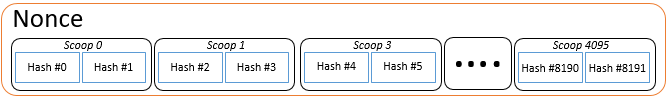
\includegraphics[width=\textwidth,keepaspectratio]{img/poc_scoops.png}
                \caption{Example of Nonce and Scoops \cite{poc}}
                \label{obr 1.2.1}
            \end{center}
        \end{minipage}
    \end{center}
\end{figure}

One of the results of the calculation will be the scoop number. This scoop number will be between 0 and 4,095. The resulting scoop number and the corresponding nonce will be used to calculate a unit of time called the “deadline”.This will be completed for all of the nonces that are on your hard drive and you will then select the shortest deadline. This minimum deadline is the amount of time that will pass since the last block was created until you can produce a new one. If the deadline that you are able to produce is shorter than those of the other miners then you are allowed to create the new block and you will be entitled to the block reward. \cite{poc}